%%%%%%%%%%%%%%%%%%%% manuscript_condensed.tex %%%%%%%%%%%%%%%%%%%%%%%%%%%%%%%%%%%
% Condensed version (~10 pages) — Springer LNCS / svproc class
%%%%%%%%%%%%%%%%%%%%%%%%%%%%%%%%%%%%%%%%%%%%%%%%%%%%%%%%%%%%%%%%%%%%%%%%%%%%%%%%%%

\documentclass[runningheads]{llncs}
\usepackage[T1]{fontenc}
\usepackage{graphicx}
\usepackage{caption}
\usepackage{subcaption}
\usepackage{float}
\usepackage{booktabs}
\usepackage{multirow}
\usepackage{array}
\usepackage{xurl}
\usepackage{amssymb}
\usepackage{amsmath}
\usepackage{makecell}
\usepackage[hidelinks]{hyperref}
\raggedbottom
\setlength{\emergencystretch}{2em}

\begin{document}

\title{A Framework for Time-Series Anomaly Detection with Mamba Backbone}
\titlerunning{A Framework for Time-Series Anomaly Detection}

%\author{Lam Huynh Khang\inst{3}, Vo Thi Ngoc Chau\inst{1,2} \and Tri Minh Pham\inst{1,2,3}}

%\institute{Ho Chi Minh City University of Technology (HCMUT)
%\and Vietnam National University, Ho Chi Minh City, Vietnam
%\and AiTA Lab, Faculty of Information Technology, FPT University
%\email{khanglhse200666@fpt.edu.vn, chauvtn@hcmut.edu.vn, tri.phamhpc@hcmut.edu.vn}}

\maketitle

\begin{abstract}
Time-series anomaly detection is important in many real-world systems such as industrial monitoring and cloud infrastructure. CARLA is a strong self-supervised framework for this task, but its ResNet backbone has limited ability to model long-range temporal patterns. We propose CARLA-MAMBA, which replaces the ResNet encoder in CARLA's pretext stage with Mamba, a selective state space model. We conduct systematic window size ablation experiments on seven benchmark datasets and find that the best window size depends on two factors: the mean sub-series length and the GPU memory limit. With properly chosen window sizes, CARLA-MAMBA substantially outperforms the original CARLA on all datasets.
\keywords{time-series, anomaly detection, contrastive learning, Mamba, state space model, self-supervised learning}
\end{abstract}

% --------------------------------------------------------------- Introduction --
\section{Introduction}
\label{sec:introduction}

Time-series anomaly detection is critical in industrial monitoring, cloud infrastructure, and cyber-physical systems. The task is difficult due to long temporal dependencies, high dimensionality, and the scarcity of labeled data \cite{darban2022deep}, which motivates self-supervised approaches.

CARLA \cite{darban2024carla} is a strong self-supervised framework with two stages: (1) contrastive representation learning via a pretext task, and (2) neighbor-based self-supervised classification. Despite strong performance, CARLA uses a ResNet backbone \cite{fawaz2019deep} designed for images. Convolutions capture local patterns well but do not model long-range temporal order.

State space models (SSMs) offer an alternative with linear complexity \cite{gu2022efficiently}. Mamba \cite{gu2023mamba} adds a selective mechanism that controls how much information is kept at each time step, enabling efficient long-range temporal modeling.

We propose \textbf{CARLA-MAMBA}, replacing the pretext-stage encoder with Mamba while keeping the rest of the pipeline unchanged for a fair comparison. We evaluate on seven benchmarks (MSL, SMAP, SMD, SWaT, WADI, Yahoo-A1, KPI) and make three contributions: (1) a Mamba-based encoder for CARLA's pretext stage; (2) a systematic window size ablation and a practical two-factor heuristic; (3) consistent improvements over the original CARLA on all seven datasets. Code: \url{https://github.com/Welkie/mamba_carla}.

% --------------------------------------------------------------- Related Work --
\section{Related Work}

\textbf{TSAD.} Anomaly detection in time series spans statistical methods (ARIMA \cite{box1970distribution}), classical ML (Isolation Forest \cite{liu2008isolation}), and deep learning \cite{schmidl2022anomaly}, including autoencoders \cite{yao2023regularizing}, VAEs \cite{park2018multimodal}, LSTMs \cite{hundman2018detecting}, and Transformers \cite{tuli2022tranad,xu2021anomaly}. Most recent work is unsupervised or self-supervised due to label scarcity \cite{pang2021deep}.

\textbf{Contrastive learning for time series.} TS2Vec \cite{yue2022ts2vec} and DCdetector \cite{yang2023dcdetector} apply contrastive objectives to time series. CARLA \cite{darban2024carla} combines anomaly injection with neighbor-based classification to achieve state-of-the-art results.

\textbf{State space models.} S4 \cite{gu2022efficiently} showed that structured SSMs handle long sequences efficiently. Mamba \cite{gu2023mamba} adds input-dependent selection and a hardware-aware parallel scan. Recent works use Mamba for time-series forecasting \cite{xu2024sst} and anomaly detection \cite{chen2024joint,sellam2025maat}.

% ---------------------------------------------------------- Materials & Methods --
\section{Materials and Methods}

\subsection{Baseline Framework: CARLA}

CARLA \cite{darban2024carla} is a two-stage self-supervised framework.

\textbf{Stage 1 (pretext):} Windows are encoded by a ResNet + MLP head. Training uses a triplet contrastive loss:
\begin{equation}
\mathcal{L}_{\text{Pretext}} = \frac{1}{|\mathcal{T}|} \sum_{(a,p,n) \in \mathcal{T}} \max\!\left(\|\phi_p(a) - \phi_p(p)\|_2^2 - \|\phi_p(a) - \phi_p(n)\|_2^2 + \alpha,\ 0\right)
\end{equation}
where $a$, $p$, $n$ are the anchor, a nearby (positive) window, and an anomaly-injected (negative) window. After training, $Q$ nearest and $Q$ furthest neighbors per window are stored.

\textbf{Stage 2 (classification):} A classifier initialized from Stage 1 is trained with:
\begin{equation}
\mathcal{L}_{\text{SS}} = \mathcal{L}_{\text{consistency}} - \mathcal{L}_{\text{inconsistency}} - \beta \cdot \mathcal{L}_{\text{entropy}}
\end{equation}
pulling windows toward nearest-neighbor predictions and pushing them from furthest neighbors. At test time, windows not in the majority (normal) class are flagged as anomalies.

\subsection{Proposed Method: CARLA-MAMBA}

We replace the Stage 1 ResNet encoder with Mamba \cite{gu2023mamba}. Mamba's core equations are:
\begin{align}
h'(t) &= \mathbf{A}h(t) + \mathbf{B}x(t), \qquad y(t) = \mathbf{C}h(t),
\end{align}
where $\mathbf{B}$, $\mathbf{C}$, and $\Delta$ depend on the current input, allowing selective retention of temporal information. Stage 2 still uses its ResNet backbone; the benefit of Mamba comes from better Stage 1 embeddings, which produce more accurate neighbor sets for Stage 2.

\begin{figure}[H]
    \centering
    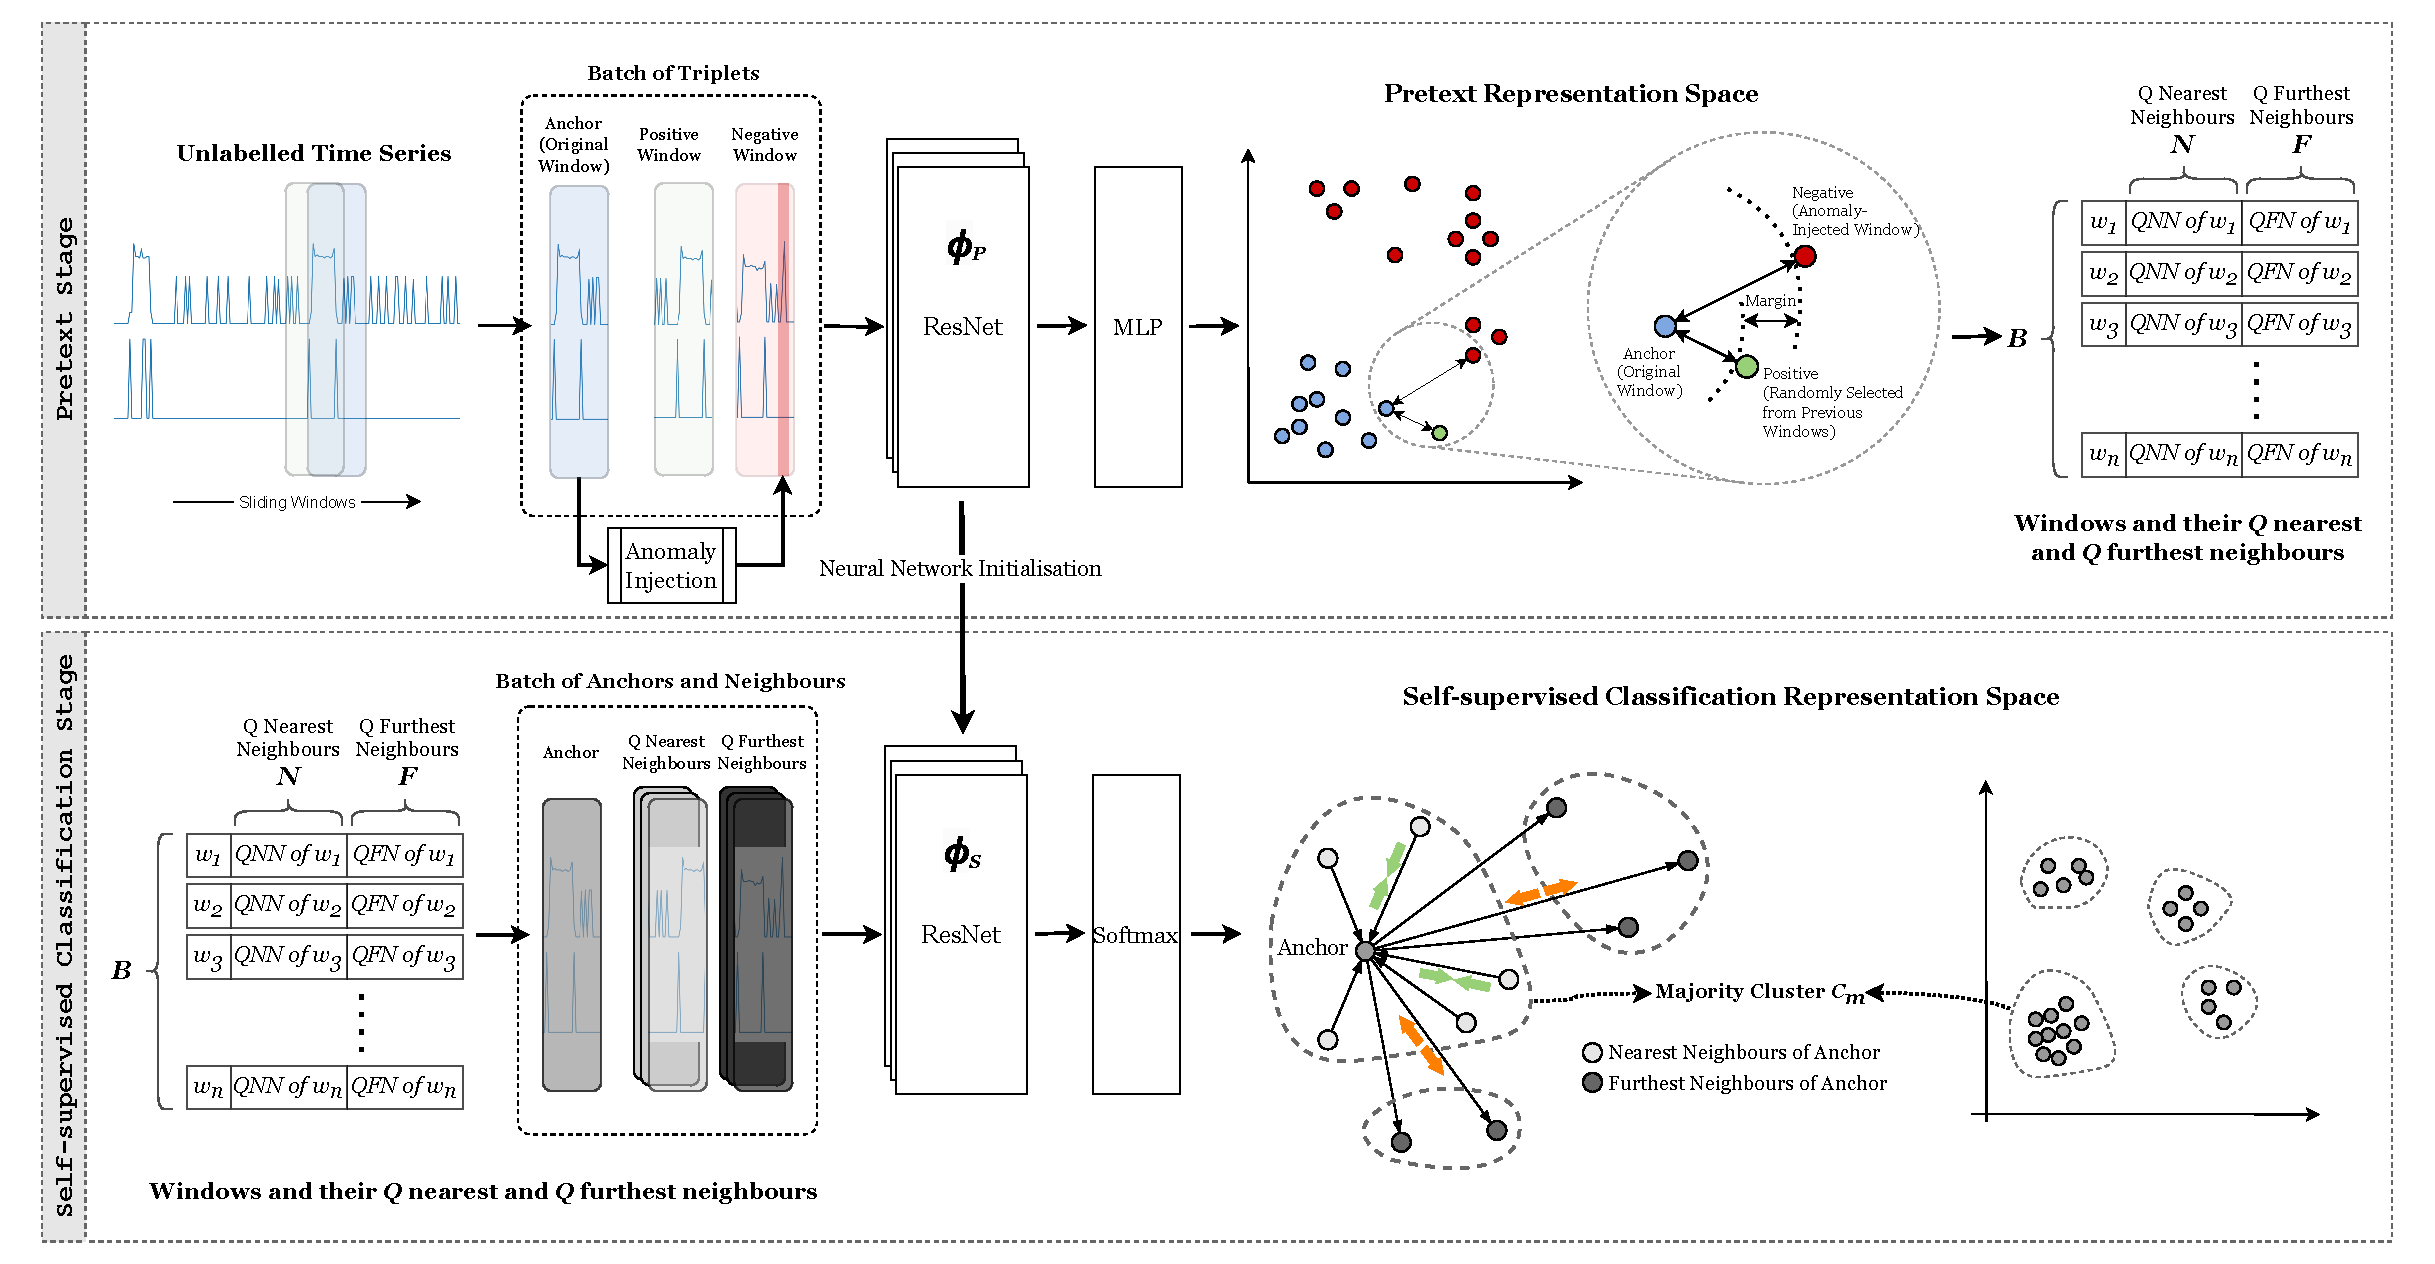
\includegraphics[
        width=0.92\linewidth,
        height=0.38\textheight,
        keepaspectratio
    ]{images/figure1_a}
    \caption{Original CARLA architecture with ResNet backbone in both stages \cite{darban2024carla}.}
    \label{fig:carla_resnet}
\end{figure}

\begin{figure}[H]
    \centering
    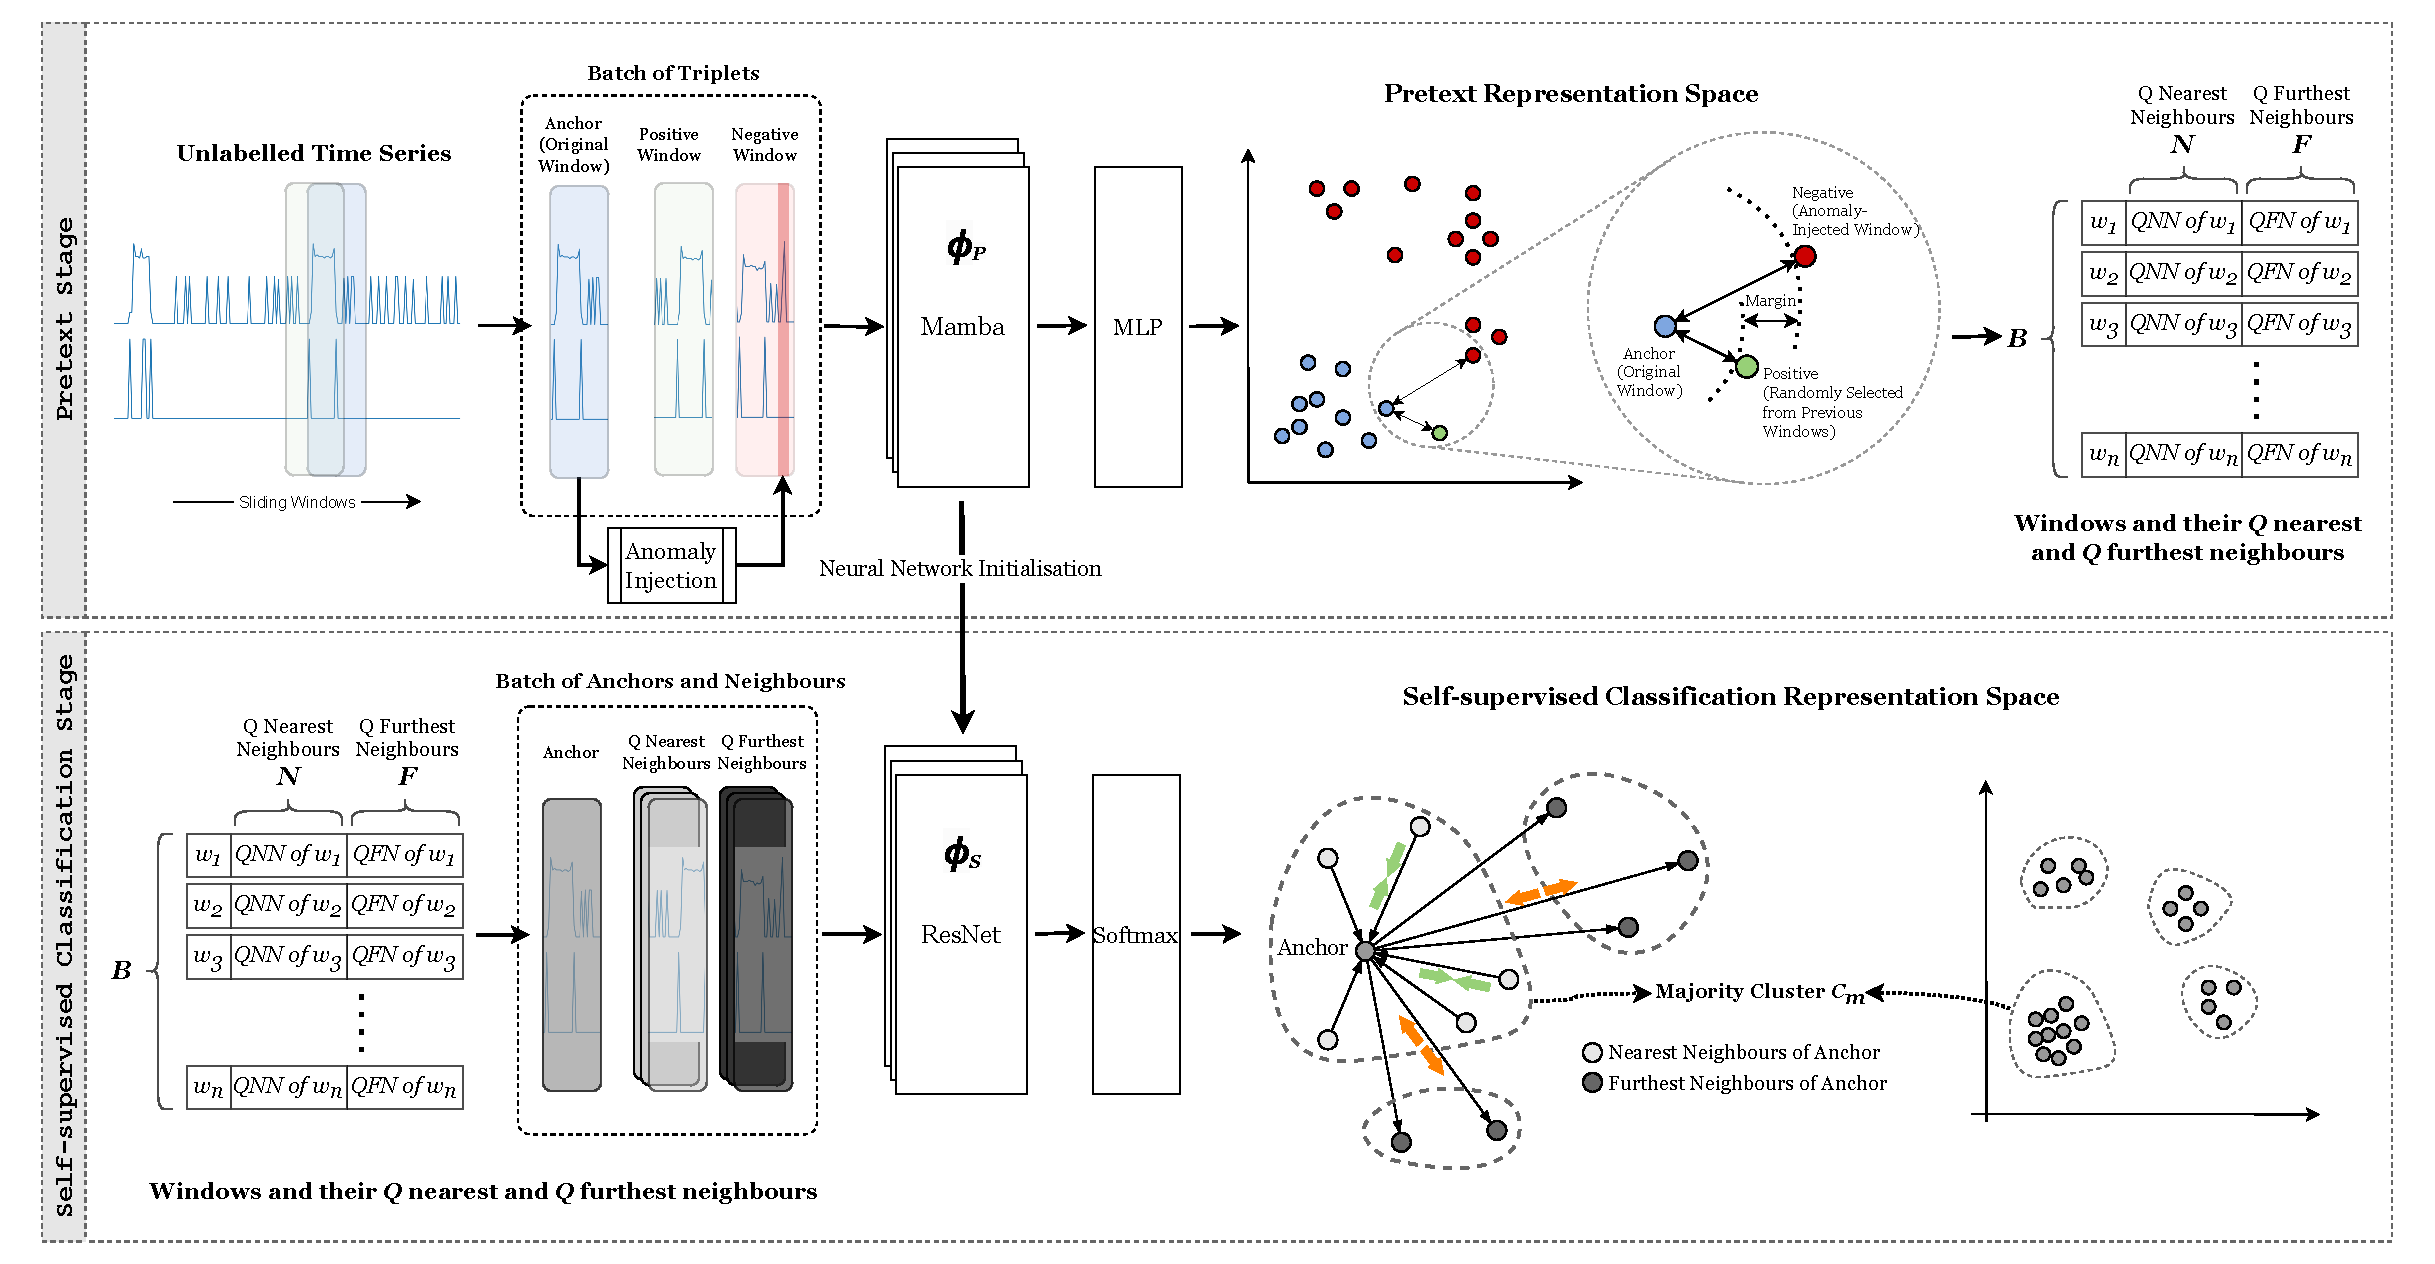
\includegraphics[
        width=0.92\linewidth,
        height=0.38\textheight,
        keepaspectratio
    ]{images/figure1_c}
    \caption{CARLA-MAMBA replaces the ResNet encoder in the pretext stage only.}
    \label{fig:carla_mamba}
\end{figure}

\subsection{Datasets and Training Protocol}

We use seven benchmark datasets (Table~\ref{tab:datasets}). All experiments run on a single NVIDIA Tesla T4 GPU (16 GB). CARLA-ResNet uses the window sizes from the original paper \cite{darban2024carla}. CARLA-MAMBA uses the best window size found by ablation (Table~\ref{tab:hyperparams}). SWaT and WADI use 10 pretext epochs; others use 30. Both variants share all other hyperparameters.

\begin{table}[htbp]
\centering
\caption{Benchmark dataset statistics.}
\label{tab:datasets}
\resizebox{\linewidth}{!}{
\begin{tabular}{lcccccc}
\toprule
\textbf{Dataset} & \textbf{\#Series} & \textbf{Dims} & \textbf{Train} & \textbf{Test} & \textbf{Anomaly(\%)} & \textbf{Ref} \\
\midrule
MSL      & 27 & 55  & 58,317    & 73,729    & 10.53 & \cite{msl_smap_dataset} \\
SMAP     & 55 & 25  & 140,825   & 444,035   & 12.85 & \cite{msl_smap_dataset} \\
SMD      & 28 & 38  & 708,405   & 708,420   &  4.16 & \cite{smd_dataset} \\
SWaT     &  1 & 51  & 496,800   & 449,919   & 12.14 & \cite{swat_dataset_kaggle} \\
WADI     &  1 & 123 & 784,568   & 172,801   &  5.77 & \cite{wadi_dataset_kaggle} \\
Yahoo-A1 & 55 &  1  & 39,096    & 39,136    &  3.79 & \cite{yahoo_a1_dataset} \\
KPI      & 29 &  1  & 1,459,418 & 1,459,429 &  2.21 & \cite{kpi_dataset} \\
\bottomrule
\end{tabular}}
\end{table}

\begin{table}[htbp]
\centering
\caption{Key hyperparameters (final configuration).}
\label{tab:hyperparams}
\resizebox{\linewidth}{!}{
\begin{tabular}{lcc}
\hline
\textbf{Parameter} & \textbf{CARLA-ResNet} & \textbf{CARLA-MAMBA} \\
\hline
Backbone (Stage 1) & ResNet (3 layers, kernels $[8,5,3]$) & Mamba (3 layers, $d\_state{=}16$, $d\_conv{=}4$, $expand{=}2$) \\
Backbone (Stage 2) & ResNet & ResNet \\
Window size (MSL / SMAP / SMD)     & 200 / 200 / 200 & 2048 / 6000 / 800 \\
Window size (SWaT / WADI)          & 200 / 400       & 128 / 2048 \\
Window size (Yahoo-A1 / KPI)       & 250 / 200       & 512 / 3100 \\
Epochs (pretext / classification)  & 30/50 (10/50 for SWaT/WADI) & same \\
Learning rate / Optimizer          & 0.001 / Adam & same \\
Batch size                         & 50 (64--256 for SWaT/WADI) & same \\
\hline
\end{tabular}}
\end{table}

\subsection{Window Size Selection Strategy}
\label{sec:window_selection}

Unlike ResNet, Mamba processes the entire input window and benefits strongly from longer temporal context. Our ablation shows that the best window size follows two factors:

\textbf{Factor 1 --- Mean series length.} For datasets with shorter sub-series (MSL, SMAP, Yahoo-A1), performance improves with window size up to a saturation point. The best window is approximately $70\%$ of the mean sub-series length $\bar{L}$:
\[
w^* \approx \rho\bar{L}, \quad \rho \approx 0.7.
\]
For example, MSL ($\bar{L}\approx2731$) peaks at $w=2048\approx0.75\bar{L}$; SMAP ($\bar{L}\approx8073$) at $w=6000\approx0.74\bar{L}$; Yahoo-A1 ($\bar{L}\approx711$) at $w=512\approx0.72\bar{L}$.

\textbf{Factor 2 --- GPU memory limit.} For long-sequence datasets (SMD, WADI, KPI), the formula above gives values that exceed GPU memory. The best practical window is:
\[
w^* = \min\!\left(\lfloor 0.7\bar{L} \rfloor,\; w_{\max}^{\text{GPU}}\right).
\]
Memory scales as $\text{Memory} \propto w \times D \times B$. SMD exceeds 16 GB beyond $w=800$, WADI beyond $w=2048$, KPI beyond $w=3100$.

\textbf{Special case.} SWaT performs best at $w=128$ despite having very long sequences. Its anomalies are short and localized; larger windows dilute the anomaly signal with normal context, reducing recall. We recommend also evaluating small windows (64--256) for datasets with localized anomalies. Table~\ref{tab:window_heuristic} validates the heuristic on all datasets.

\begin{table}[htbp]
\centering
\caption{Validation of the proposed window size heuristic.}
\label{tab:window_heuristic}
\resizebox{\linewidth}{!}{
\begin{tabular}{lcccc}
\hline
\textbf{Dataset} & $\mathbf{\bar{L}}$ & $\mathbf{0.7\bar{L}}$ & \textbf{Selected $w^*$} & \textbf{Dominant Factor} \\
\hline
MSL      & 2,731   & 1,911   & 2048 & Long-context beneficial \\
SMAP     & 8,073   & 5,651   & 6000 & Long-context beneficial \\
Yahoo-A1 & 711     & 497     & 512  & Long-context beneficial \\
SMD      & 25,300  & 17,710  & 800  & GPU memory limit \\
WADI     & 172,801 & 120,960 & 2048 & GPU memory limit \\
KPI      & 50,325  & 35,227  & 3100 & GPU memory limit \\
SWaT     & 449,919 & 314,943 & 128  & Localized anomalies \\
\hline
\end{tabular}}
\end{table}

\subsection{Evaluation Metrics}

We report Precision, Recall, F1-score, AU-PR, total inference time, and peak GPU memory. Point Adjustment (PA) is not used as it can overestimate performance \cite{kim2022towards}.

% --------------------------------------------------------------- Results --
\section{Results}
\label{sec:results}

\subsection{Overall Performance}

Table~\ref{tab:carla_comparison} shows the final comparison. CARLA-MAMBA outperforms CARLA-ResNet on all seven datasets in both F1-score and AU-PR. The largest gains are on SMAP (F1: $0.54{\to}1.00$) and MSL (F1: $0.53{\to}0.98$). Large improvements also appear on KPI ($0.25{\to}0.81$), WADI ($0.35{\to}0.65$), SWaT ($0.69{\to}0.94$), SMD ($0.41{\to}0.62$), and Yahoo-A1 ($0.81{\to}0.89$). Figure~\ref{fig:combined_results} visualizes the comparison. These results confirm that Mamba needs sufficient temporal context: with a small window it often underperforms ResNet, but after increasing the window appropriately, performance improves substantially across all benchmarks.

\begin{figure}[H]
  \centering
  \begin{subfigure}[t]{0.48\linewidth}
    \centering
    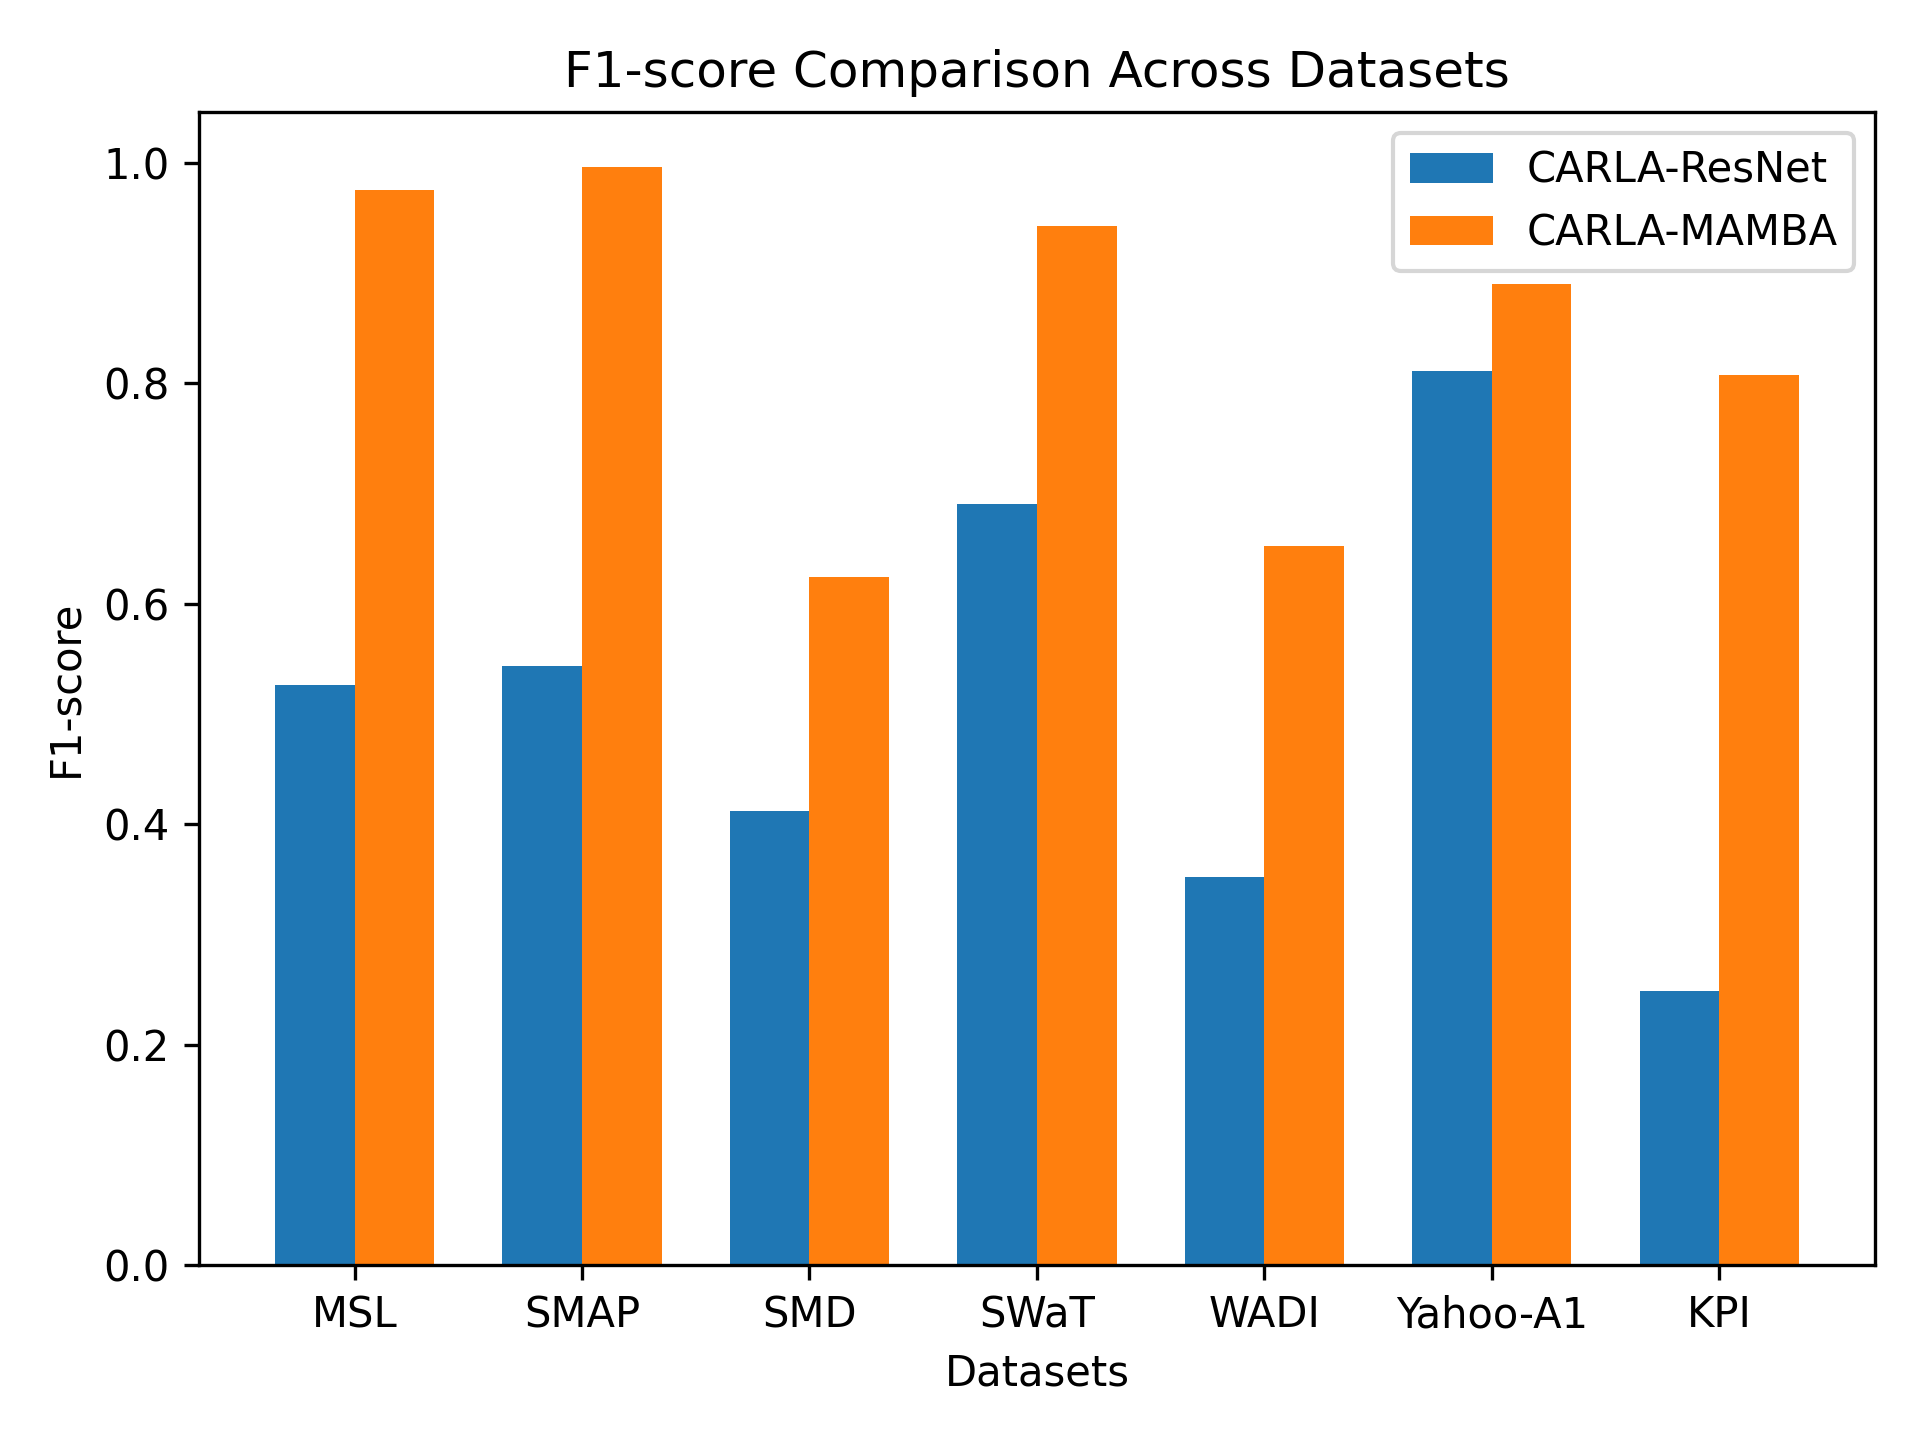
\includegraphics[width=\linewidth]{images/f1_comparison.png}
    \caption{F1-score}
  \end{subfigure}
  \hfill
  \begin{subfigure}[t]{0.48\linewidth}
    \centering
    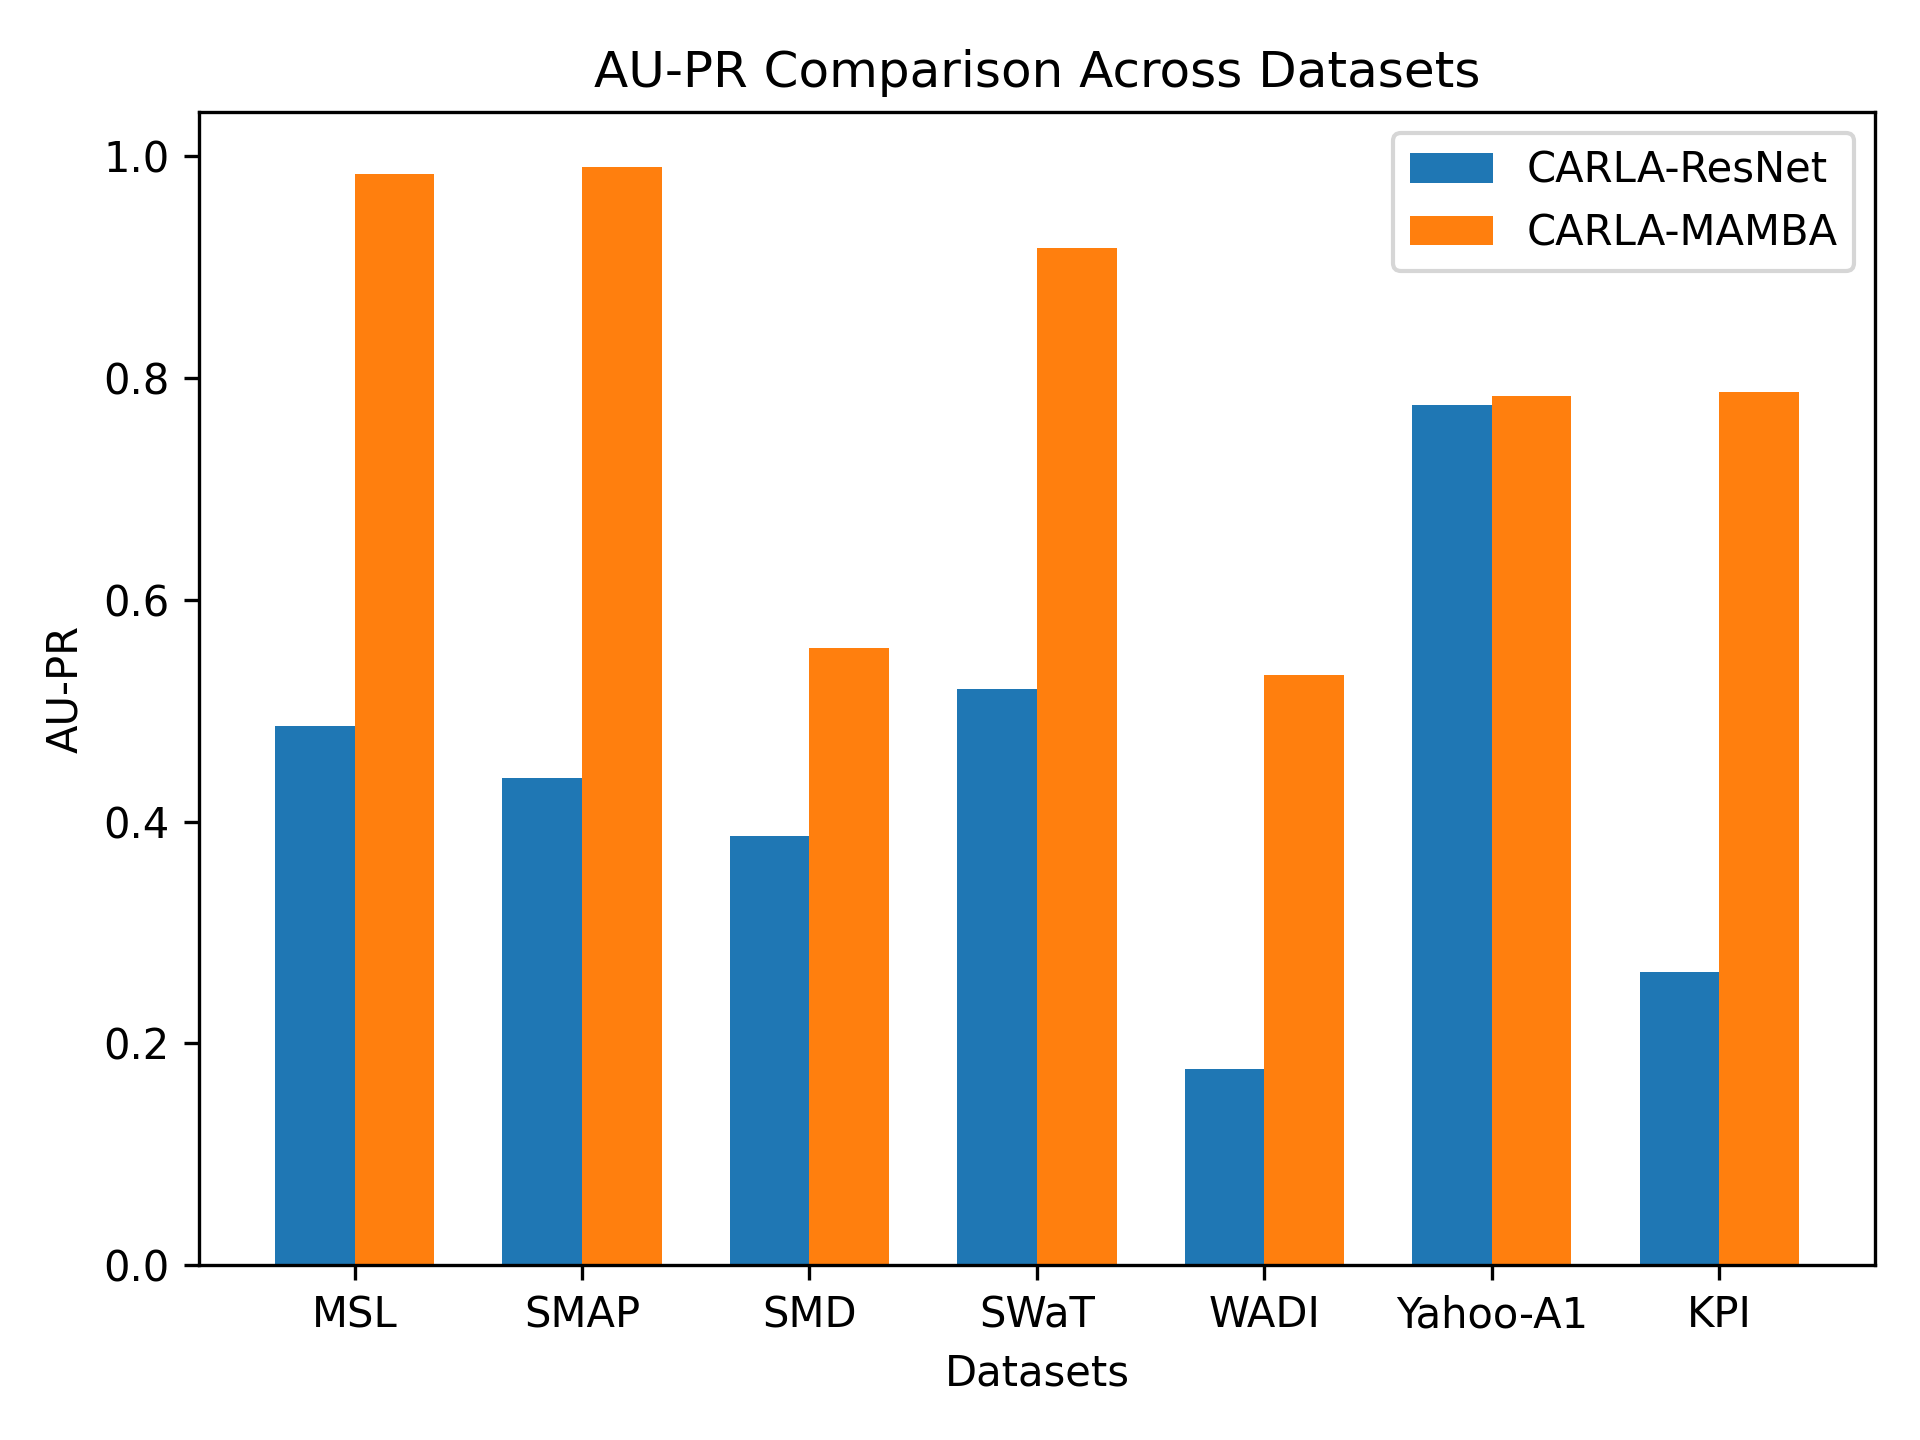
\includegraphics[width=\linewidth]{images/aupr_comparison.png}
    \caption{AU-PR}
  \end{subfigure}
  \caption{CARLA-ResNet vs.\ CARLA-MAMBA across seven datasets.}
  \label{fig:combined_results}
\end{figure}

\begin{table}[htbp]
\centering
\caption{Final comparison using the best window size per dataset.}
\label{tab:carla_comparison}
\resizebox{\linewidth}{!}{
\begin{tabular}{llccccccc}
\hline
\textbf{Dataset} & \textbf{Method} & \textbf{Prec} & \textbf{Rec} & \textbf{F1} & \textbf{AU-PR} & \textbf{Time (s)} & \textbf{Avg./Series (s)} & \textbf{Mem.(MB)} \\
\hline
\multirow{2}{*}{MSL}
 & ResNet & 0.3910 & 0.8025 & 0.5258 & $0.4866{\pm}0.2519$ & 12351.98 & 457.48 & 1230.80 \\
 & MAMBA  & \textbf{0.9630} & \textbf{0.9873} & \textbf{0.9750} & $\mathbf{0.9838{\pm}0.0469}$ & 5598.14 & 207.34 & 6859.53 \\
\hline
\multirow{2}{*}{SMAP}
 & ResNet & 0.4233 & 0.7589 & 0.5435 & $0.4396{\pm}0.3217$ & 33924.34 & 616.81 & 382.69 \\
 & MAMBA  & \textbf{0.9923} & \textbf{1.0000} & \textbf{0.9961} & $\mathbf{0.9905{\pm}0.0676}$ & 14015.99 & 254.84 & 1176.30 \\
\hline
\multirow{2}{*}{SMD}
 & ResNet & 0.3144 & 0.5987 & 0.4123 & $0.3870{\pm}0.1908$ & 33763.76 & 1205.85 & 1540.48 \\
 & MAMBA  & \textbf{0.4835} & \textbf{0.8804} & \textbf{0.6242} & $\mathbf{0.5564{\pm}0.1856}$ & 35260.63 & 1259.31 & 5926.61 \\
\hline
\multirow{2}{*}{SWaT}
 & ResNet & 0.7917 & 0.6126 & 0.6908 & 0.5193 & 1142.35 & 1142.35 & 206.96 \\
 & MAMBA  & \textbf{1.0000} & \textbf{0.8909} & \textbf{0.9423} & \textbf{0.9175} & 1190.11 & 1190.11 & 623.77 \\
\hline
\multirow{2}{*}{WADI}
 & ResNet & 0.2202 & 0.8824 & 0.3525 & 0.1771 & 1496.77 & 1496.77 & 179.48 \\
 & MAMBA  & \textbf{0.4840} & \textbf{1.0000} & \textbf{0.6523} & \textbf{0.5322} & 2877.58 & 2877.58 & 1127.98 \\
\hline
\multirow{2}{*}{Yahoo-A1}
 & ResNet & 0.6946 & 0.9746 & 0.8111 & $0.7761{\pm}0.3397$ & 5609.75 & 102.00 & 42.39 \\
 & MAMBA  & \textbf{0.8047} & \textbf{0.9948} & \textbf{0.8897} & $\mathbf{0.7835{\pm}0.3677}$ & 3444.70 & 62.63 & 165.87 \\
\hline
\multirow{2}{*}{KPI}
 & ResNet & 0.1500 & 0.7206 & 0.2483 & $0.2644{\pm}0.2343$ & 62356.69 & 2150.23 & 371.06 \\
 & MAMBA  & \textbf{0.6887} & \textbf{0.9768} & \textbf{0.8078} & $\mathbf{0.7879{\pm}0.2227}$ & 80907.62 & 2789.92 & 1715.25 \\
\hline
\end{tabular}}
\end{table}

\subsection{Window Size Ablation}

Table~\ref{tab:ablation} shows detailed ablation results. For most datasets, F1 increases with window size until GPU memory is exhausted (OOM). SWaT is the exception: F1 drops sharply after $w=128$, confirming that localized anomalies require small windows. On MSL, SMAP, and Yahoo-A1, larger windows also reduce inference time by cutting the total number of overlapping windows, but increase GPU memory substantially.

\begin{table}[H]
\centering
\caption{Window size ablation results on seven benchmark datasets.
Entries marked \textsf{---} were not evaluated.
\textsf{OOM} indicates configurations that exceeded
the 16\,GB Tesla T4 memory limit.
Bold rows indicate the best-performing configuration per dataset.}
\label{tab:ablation}
\resizebox{\linewidth}{!}{%
\begin{tabular}{lllccccccc}
\toprule
\textbf{Dataset} &
\textbf{Method} &
\textbf{wsz} &
\textbf{Prec} & \textbf{Rec} & \textbf{F1} & \textbf{AU-PR} &
\textbf{Time (s)} & \textbf{Avg./Series (s)} & \textbf{Mem.(MB)} \\
\midrule

\multirow{7}{*}{MSL}
 & ResNet & 200   & 0.3910 & 0.8025 & 0.5258 & $0.4866\pm0.2519$ & 12351.98 & 457.48 & 1230.80 \\
 & Mamba  & 128   & \textsf{---} & \textsf{---} & \textsf{---} & \textsf{---} & \textsf{---} & \textsf{---} & \textsf{---} \\
 & Mamba  & 256   & 0.4196 & 0.8048 & 0.5516 & $0.5126\pm0.2327$ & 12056.33 & 446.53 & 1549.12 \\
 & Mamba  & 512   & 0.6132 & 0.8487 & 0.7120 & $0.6987\pm0.1693$ & 10789.86 & 399.62 & 2884.31 \\
 & Mamba  & 1024  & 0.8186 & 0.9488 & 0.8789 & $0.8286\pm0.1703$ &  8939.50 & 331.09 & 4978.65 \\
 & \textbf{Mamba}  & \textbf{2048}  & \textbf{0.9630} & \textbf{0.9873} & \textbf{0.9750} & $\mathbf{0.9838\pm0.0469}$ &  5598.14 & 207.34 & 6859.53 \\
 & Mamba  & 4096  & 0.9576 & 0.9916 & 0.9743 & $0.9851\pm0.0469$ &  4440.39 & 164.46 & 5838.87 \\
\midrule

\multirow{8}{*}{SMAP}
 & ResNet & 200   & 0.4233 & 0.7589 & 0.5435 & $0.4396\pm0.3217$ & 33924.34 & 616.81 & 382.69 \\
 & Mamba  & 128   & 0.2756 & 0.8260 & 0.4133 & $0.3168\pm0.3065$ & 36051.42 & 655.48 & 369.43 \\
 & Mamba  & 256   & 0.3189 & 0.8322 & 0.4611 & $0.3663\pm0.3137$ & 30623.82 & 556.80 & 469.62 \\
 & Mamba  & 512   & \textsf{---} & \textsf{---} & \textsf{---} & \textsf{---} & \textsf{---} & \textsf{---} & \textsf{---} \\
 & Mamba  & 1024  & 0.3586 & 0.9061 & 0.5138 & $0.3806\pm0.2760$ & 30044.19 & 546.26 & 1297.81 \\
 & Mamba  & 2048  & 0.5749 & 0.9275 & 0.7098 & $0.5836\pm0.2511$ & 18645.16 & 339.00 & 1176.39 \\
 & Mamba  & 4096  & 0.8338 & 0.9874 & 0.9041 & $0.8121\pm0.1936$ & 19155.87 & 348.29 & 1176.35 \\
 & \textbf{Mamba}  & \textbf{6000}  & \textbf{0.9923} & \textbf{1.0000} & \textbf{0.9961} & $\mathbf{0.9905\pm0.0676}$ & 14015.99 & 254.84 & 1176.30 \\
\midrule

\multirow{6}{*}{SMD}
 & ResNet & 200   & 0.3144 & 0.5987 & 0.4123 & $0.3870\pm0.1908$ & 33763.76 & 1205.85 & 1540.48 \\
 & Mamba  & 128   & \textsf{---} & \textsf{---} & \textsf{---} & \textsf{---} & \textsf{---} & \textsf{---} & \textsf{---} \\
 & Mamba  & 256   & \textsf{---} & \textsf{---} & \textsf{---} & \textsf{---} & \textsf{---} & \textsf{---} & \textsf{---} \\
 & Mamba  & 512   & 0.3884 & 0.8340 & 0.5300 & $0.4401\pm0.1808$ & 33093.38 & 1181.91 & 3840.36 \\
 & \textbf{Mamba}  & \textbf{800}   & \textbf{0.4835} & \textbf{0.8804} & \textbf{0.6242} & $\mathbf{0.5564\pm0.1856}$ & 35260.63 & 1259.31 & 5926.61 \\
 & Mamba  & 1024  & \multicolumn{7}{c}{\textsf{OOM}} \\
\midrule

\multirow{5}{*}{SWaT}
 & ResNet & 200   & 0.7917 & 0.6126 & 0.6908 & 0.5193 & 1142.35 & 1142.35 & 206.96 \\
 & Mamba  & 64    & 0.9866 & 0.8764 & 0.9282 & 0.9442 &  943.38 &  943.38 & 189.02 \\
 & \textbf{Mamba}  & \textbf{128}   & \textbf{1.0000} & \textbf{0.8909} & \textbf{0.9423} & \textbf{0.9175} & 1190.11 & 1190.11 & 623.77 \\
 & Mamba  & 256   & 1.0000 & 0.5907 & 0.7427 & 0.6457 & 1124.73 & 1124.73 & 467.78 \\
 & Mamba  & 512   & 1.0000 & 0.3379 & 0.5051 & 0.4196 & 1478.38 & 1478.38 & 914.62 \\
\midrule

\multirow{7}{*}{WADI}
 & ResNet & 400   & 0.2202 & 0.8824 & 0.3525 & 0.1771 & 1496.77 & 1496.77 & 179.48 \\
 & Mamba  & 128   & \textsf{---} & \textsf{---} & \textsf{---} & \textsf{---} & \textsf{---} & \textsf{---} & \textsf{---} \\
 & Mamba  & 256   & \textsf{---} & \textsf{---} & \textsf{---} & \textsf{---} & \textsf{---} & \textsf{---} & \textsf{---} \\
 & Mamba  & 512   & 0.2298 & 0.7314 & 0.3497 & 0.1959 & 1433.61 & 1433.61 & 297.37 \\
 & Mamba  & 1024  & 0.3226 & 1.0000 & 0.4878 & 0.3056 & 1661.55 & 1661.55 & 569.73 \\
 & \textbf{Mamba}  & \textbf{2048}  & \textbf{0.4840} & \textbf{1.0000} & \textbf{0.6523} & \textbf{0.5322} & 2877.58 & 2877.58 & 1127.98 \\
 & Mamba  & 2300  & \multicolumn{7}{c}{\textsf{OOM}} \\
\midrule

\multirow{5}{*}{Yahoo-A1}
 & ResNet & 250   & 0.6946 & 0.9746 & 0.8111 & $0.7761\pm0.3397$ &  5609.75 & 102.00 &  42.39 \\
 & Mamba  & 128   & 0.4707 & 0.9546 & 0.6305 & $0.6157\pm0.3447$ &  8070.21 & 146.73 & 165.65 \\
 & Mamba  & 256   & 0.5864 & 0.9867 & 0.7356 & $0.6355\pm0.3941$ &  5845.12 & 106.27 &  92.93 \\
 & \textbf{Mamba}  & \textbf{512}   & \textbf{0.8047} & \textbf{0.9948} & \textbf{0.8897} & $\mathbf{0.7835\pm0.3677}$ &  3444.70 &  62.63 & 165.87 \\
 & Mamba  & 1024  & 0.7964 & 0.9948 & 0.8846 & $0.7705\pm0.3769$ &  3155.92 &  57.38 & 165.87 \\
\midrule

\multirow{7}{*}{KPI}
 & ResNet & 200   & 0.1500 & 0.7206 & 0.2483 & $0.2644\pm0.2343$ & 62356.69 & 2150.23 &  371.06 \\
 & Mamba  & 128   & \textsf{---} & \textsf{---} & \textsf{---} & \textsf{---} & \textsf{---} & \textsf{---} & \textsf{---} \\
 & Mamba  & 256   & \textsf{---} & \textsf{---} & \textsf{---} & \textsf{---} & \textsf{---} & \textsf{---} & \textsf{---} \\
 & Mamba  & 512   & 0.2453 & 0.8415 & 0.3798 & $0.3235\pm0.2276$ & 66186.61 & 2282.30 &  316.46 \\
 & Mamba  & 1024  & 0.3766 & 0.9352 & 0.5369 & $0.4664\pm0.2278$ & 73381.32 & 2530.39 &  596.48 \\
 & \textbf{Mamba}  & \textbf{3100}  & \textbf{0.6887} & \textbf{0.9768} & \textbf{0.8078} & $\mathbf{0.7879\pm0.2227}$ & 80907.62 & 2789.92 & 1715.25 \\
 & Mamba  & 4096  & \multicolumn{7}{c}{\textsf{OOM}} \\

\bottomrule
\end{tabular}%
}
\end{table}

% --------------------------------------------------------------- Discussion --
\section{Discussion}
 
\textbf{Why Mamba improves CARLA.}
ResNet captures local patterns through small convolution kernels, limiting its ability to model information across large temporal intervals. Mamba processes the full sequence and decides at each step which information to keep, producing embeddings that better separate normal from anomalous patterns. Because Stage 2 depends on the neighbor sets from Stage 1, better Stage 1 representations lead to stronger detection boundaries — an effect especially large on MSL, SMAP, and KPI.
 
\textbf{Window size and anomaly locality.}
For datasets with distributed anomalies (MSL, SMAP, KPI), larger windows improve F1 almost monotonically until saturation. For SWaT, whose anomalies are short and localized, larger windows mix anomaly events with too much normal context, reducing recall significantly. The optimal window therefore depends on both sequence length and anomaly locality: long-range structures favor large windows, while localized patterns prefer compact context.
 
\textbf{Performance vs.\ memory trade-off.}
Large windows improve F1 but greatly increase GPU memory. On MSL, the best configuration (w=2048) uses 6.8 GB vs.\ 1.2 GB for ResNet, while inference time drops from 12351.98 s to 5598.14 s due to fewer overlapping windows. In practice, $w^* = \min(\lfloor 0.7\bar{L} \rfloor, w_{\max}^{\text{GPU}})$ is a reliable starting point, with additional small-window evaluation for datasets with localized anomalies.
 
\textbf{Limitations.}
Experiments are limited to a single 16 GB GPU and a single random seed. The heuristic requires empirical validation for new datasets when anomaly locality is unknown. Only Stage 1 is replaced; exploring hybrid architectures or modifying both stages may improve performance further.

% --------------------------------------------------------------- Conclusion --
\section{Conclusion}

In this paper, we proposed CARLA-MAMBA, a modified version of the CARLA framework where the ResNet backbone in the pretext stage is replaced with Mamba, a selective state space model designed for efficient long-sequence modeling.

We conducted extensive experiments on seven benchmark datasets and performed systematic window size ablation studies. The results show that window size is a critical factor for Mamba-based time-series anomaly detection.

When the temporal window is properly selected, CARLA-MAMBA consistently outperforms the original CARLA baseline across all seven benchmark datasets in both F1-score and AU-PR.

Our experiments also reveal a strong relationship between dataset characteristics and optimal window size. Datasets with long temporal dependencies benefit significantly from large windows, while datasets with highly local anomalies prefer smaller temporal context.

These findings demonstrate that Mamba is a highly effective backbone for self-supervised time-series anomaly detection when sufficient temporal context is available.

Future work will focus on developing theoretically grounded automatic window selection methods, memory-efficient long-sequence training strategies, and hybrid architectures that combine local convolutional modeling with global state space modeling. We also plan to investigate newer selective state space models such as Mamba-2 and multi-stage sequence modeling architectures for anomaly detection.

\section*{Declaration}
Declaration of generative AI and AI-assisted technologies in the writing process ChatGPT was used for assisting with language editing only. The authors reviewed and revised the manuscript and take full responsibility for the accuracy and integrity of the work.

\bibliographystyle{splncs03_unsrt}
\bibliography{references}

\end{document}